\section{Theoretischer Hintergrund}
\label{sec:Theorie}

\subsection{Eigenschaften des Myons}
\label{subsec:Eigenschaften}

Myonen sind Leptonen aus der zweiten der drei Leptonenfamilien. Sie haben
eine Ruhemasse von $\SI{105.66}{\mega\electronvolt}$ sowie eine Lebensdauer
von $\SI{2.197}{\micro\second}$. Das Myon $\mu^{-}$ ist einfach negativ geladen,
das Antimyon $\mu^{+}$ daher einfach positiv.
Myonen unterliegen wie alle Fermionen der schwachen und der elektromagnetischen
Wechselwirkung.

\subsection{Enstehung von kosmischer Strahlung}
\label{subsec:kosmischeStrahlung}



Myonen zerfallen wie folgt über die schwache Wechselwirkung:
\begin{figure}
  \centering
  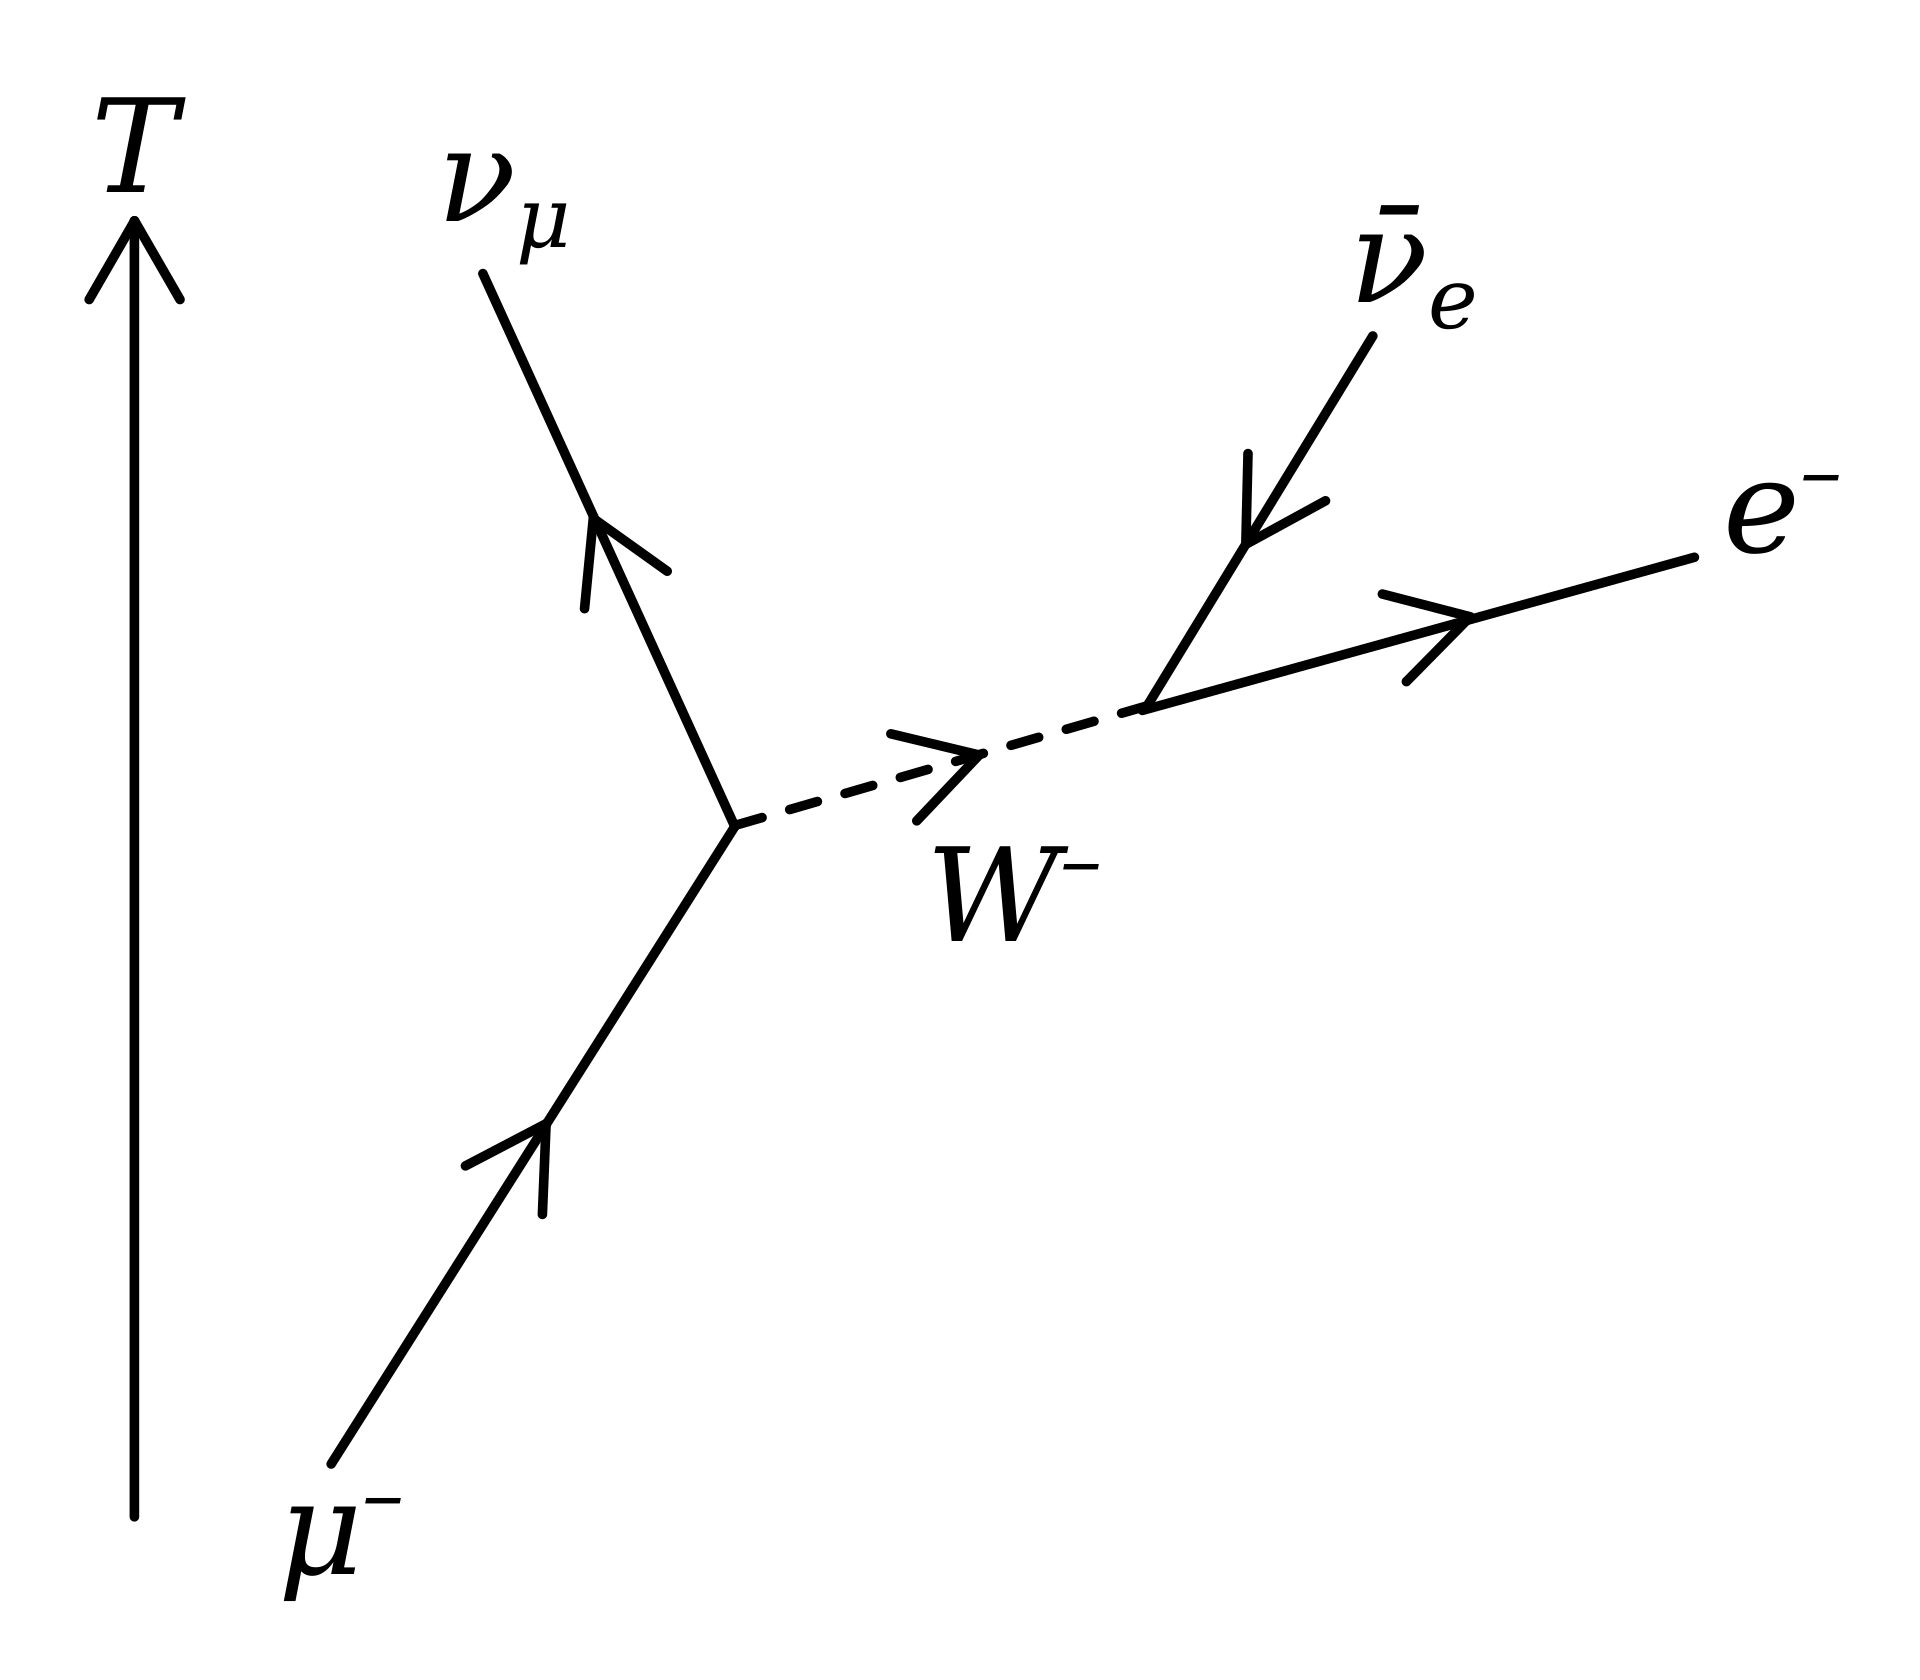
\includegraphics[width=0.5\textwidth]{pictures/Muon_Decay.png}
  \caption{Feynman-Graph des Myonenzerfalls.\cite{Myon-Wikipedia}}
  \label{zerfall}
\end{figure}

